\section[\thesection \  Training]{Training}\label{sec:training}
%
%--------------------------------------------------------------------
%


\subsection[\thesection .\thesubsection \ 
Sammeln und Aufbereiten der Daten]{Sammeln und Aufbereiten der Daten}\label{subsec:collect_data}
\begin{frame}{Datensatz}
   
   Bilder + Labels mit Koordinaten der Bounding Boxen

    \begin{itemize}
        \item \textbf{OpenImages} Open Source Dataset von Google
    \end{itemize}
    \begin{itemize}
        \item 9 Klassen mit Wildtieren (je 200 bis 2000 Bilder)
        \begin{itemize}
            \item Braun Bär, Hirsch, Fuchs, Ziege, Igel, Eule, Hase, Waschbär, Eichhörnchen
        \end{itemize}
    \end{itemize}
    \vspace{0.5cm}
    
\visible<2->{

    \begin{block}{Validierung und Overfitting}
        Kontrolle des Trainings durch Aufteilen der Daten in:
        \begin{figure}[h]
            \centering
            \def\svgwidth{0.8\columnwidth}
            \input{Bilder/train_test_val.pdf_tex}
        \end{figure}
        \begin{itemize}
            \item \textbf{Overfitting:} Nur die Trainingsdaten werden gelernt
        \end{itemize}
    \end{block}

    }
\end{frame}

\begin{frame}{Augmentierung}
    Künstlich mehr Daten erzeugen, verhindern von Overfitting
        \begin{figure}
            \centering
            \includegraphics[width=0.6\textwidth]{Bilder/augmentierung.png}            
        \end{figure}
        \begin{itemize}
            \item Geometrisch: Verschieben, Spiegeln, Rotieren, Zoom
            \item oder: Farbwerte, Helligkeit, Kontrast, Rauschen, Dropout
        \end{itemize}

\end{frame}

\subsection[\thesection .\thesubsection \ 
Auswahl und Training des Modells]{Auswahl und Training des Modells}\label{subsec:train}


\begin{frame}{Convolutional Neural Network}
    \begin{columns}[T]
        \column{0.3\columnwidth}
        \begin{itemize}
            \item Faltung des Inputs mit Filter Matrix
        \end{itemize}
        \begin{itemize}
            \item Erzeugen Feature-Maps
        \end{itemize}
        \begin{itemize}
            \item Räumliche Invarianz
        \end{itemize}
        \vspace{0.5cm}
        
        \column{0.7\columnwidth}
        \begin{figure}
            \centering
            \def\svgwidth{0.95\columnwidth}
            \input{Bilder/lenet.pdf_tex}
        \end{figure}
        
    \end{columns}
    \visible<2->{
    

    \begin{columns}[T]
    \column{0.45\columnwidth}


    \begin{block}{Objekt Detection}
            \begin{itemize}
                \item Basis CNN
                \begin{itemize}
                    \item Feature Extraction                    
                \end{itemize}
            \end{itemize}        
            \begin{itemize}
                \item Object Detection Framework
                \begin{itemize}
                    \item Single Shot Det. (SSD)
                    \item Region Based (R-CNN)
                \end{itemize}
            \end{itemize}
        \end{block}
            \column{0.55\columnwidth}
            
            \begin{figure}
                \centering
                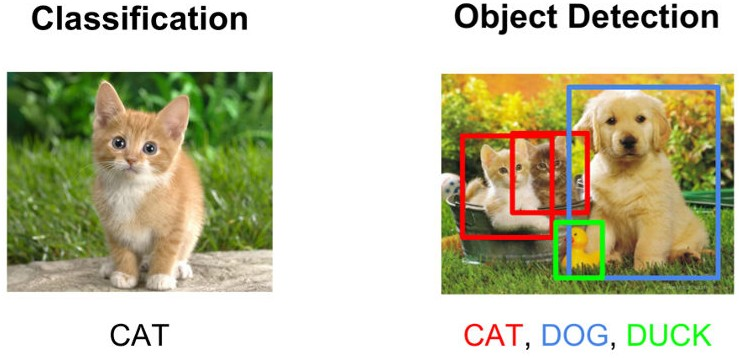
\includegraphics[width=\textwidth]{Bilder/classification_detection.jpeg}
            \end{figure}
        \end{columns}
    }
\end{frame}

\begin{frame}{Trainingsworkflow}
    Framework: \textit{Tensorflow}
    \\[0.3cm]
    Mehrfaches Durchlaufen und anpassen des Trainingsprozess
    \begin{figure}
        \centering
            \def\svgwidth{0.9\columnwidth}
            
\tikzstyle{process} = [rectangle, fill=blue!20, node distance=4cm, minimum width=1.5cm, minimum height=0.8cm, text centered, draw=black]
\tikzstyle{arrow} = [thick,->,>=stealth]
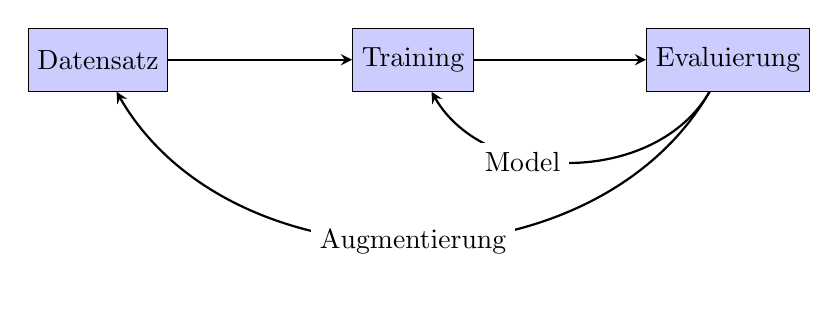
\begin{tikzpicture}[scale=0.4]
      \node (data)      [process]                   {Datensatz};
      \node (train)      [process, right of=data]      {Training};
      \node (eval)      [process, right of=train]      {Evaluierung};
    \draw[arrow] (data) -- (train);
    \draw[arrow] (train) -- (eval);
  \draw[arrow] (eval) edge[bend left=60] node [centered, fill=white!30] {Augmentierung} (data);
  \draw[arrow] (eval) edge[bend left=60] node [left, fill=white!30] {Model} (train);
\end{tikzpicture}

% \begin{tikzpicture}[scale=0.4]

%   \begin{scope}[node distance=3cm]

%    \node (data)      [process]                   {Datensatz};
%    \node (prep)      [process, right of=data]      {Aufbereitung};
%    \node (model)      [process, right of=prep]      {Model};
%    \node (train)      [process, right of=model]      {Training};
%    \node (eval)      [process, right of=train]      {Evaluierung};

%   \end{scope}

%  \draw[arrow] (data) -- (prep);
%  \draw[arrow] (prep) -- (model);
%  \draw[arrow] (model) -- (train);
%  \draw[arrow] (train) -- (eval);
 

% \draw[arrow] (eval) edge[bend left=60] node [left, fill=white!30] {ändern} (data);
% \draw[arrow] (eval) edge[bend left=60] node [left, fill=white!30] {augment} (prep);
% \draw[arrow] (eval) edge[bend left=60] node [left, fill=white!30] {ändern} (model);
% \draw[arrow] (eval) edge[bend left=60] node [left, fill=white!30] {Parameter} (train);

 
% \end{tikzpicture}

    \end{figure}
    \visible<2->{
        \begin{columns}[T]
            \column{0.3\columnwidth}
            \begin{itemize}
            \item Datensatz
            \begin{itemize}
                \item Augmentierung
                \item Graustufen
            \end{itemize}
            \end{itemize}
            \column{0.3\columnwidth}
            \begin{itemize}
                \item Modelle:
                \begin{itemize}
                    \item Faster R-CNNs
                    \item SSDs
                \end{itemize}
            \end{itemize}
            \column{0.4\columnwidth}
            \begin{itemize}
                \item Evaluierung:
                \begin{itemize}
                    \item Genauigkeit (mAP)
                    \item Fehlerrate (Loss)
                \end{itemize}
            \end{itemize}
        \end{columns}
    }
\end{frame}

